\RequirePackage{pdfmanagement}
\SetKeys[document/metadata]{pdfversion=1.7, pdfstandard=A-2u, lang=en-GB}
\input{preamble/pdfA-compliance/glyphtounicode}
\documentclass[11pt,a4paper]{report}
\newcommand*{\PaperTitle}{A computer-assisted proof of the critical-parameter conjecture for the perturbed Gelfand equation on the disk}
\newcommand*{\PaperTitlePlain}{A computer-assisted proof of the critical-parameter conjecture for the perturbed Gelfand equation on the disk}
\newcommand*{\PaperShortTitle}{The critical Gelfand parameter}
\newcommand*{\PaperSubtitle}{chemistry-open-problems \textperiodcentered{} 18 October 2026 \textperiodcentered{} solved}
\newcommand*{\PaperCredits}{Solver: GPT-6-Astra (effort xhigh) \textperiodcentered{} Verifier: Claude Opus 5.5 (effort xhigh), confirmed with corrections}
\newcommand*{\PaperKeywords}{perturbed Gelfand equation, cusp, validated ODE integration, combustion}
\input{chemop-preamble}
\addbibresource{references.bib}

\begin{document}
\makepapertitle
\begin{paperabstract}
We give a computer-assisted proof of the critical-parameter conjecture for the
two-dimensional perturbed Gelfand equation. There is a unique critical value
$\varepsilon_0$ within $10^{-12}$ of $0.24210616559524695$: every curve below it
is exactly S-shaped, and every curve at or above it is strictly increasing.
At equality the derivative has one double zero. The Du--Lou change of variables
turns the entire fold set into the stopping-level curve of a single shooting
family. A Wronskian identity handles arbitrarily small transformed amplitudes; a
validated cover of 110 intervals handles the compact remainder; the known
limiting-problem theorem of Du and Lou excludes the tail. A separate 160-bit Arb
contraction certifies the cusp. Every integration includes rigorous origin and
remainder bounds. An independent verifier re-derived the reduction, re-ran all
certificates and reproduced the cover, the critical value and the cusp with a
separate validated integrator; see \texttt{verification.md}.
\end{paperabstract}

\section*{The open question and prior work}
We consider positive solutions of
\begin{equation}\label{eq:pde}
 \Delta u+\lambda\exp\!\left(\frac{u}{1+\varepsilon u}\right)=0
 \quad\text{in }B_1\subset\mathbb R^2,\qquad u|_{\partial B_1}=0,
 \qquad \lambda,\varepsilon>0.
\end{equation}
Korman, Li and Ouyang, arXiv:1612.07722, printed page 3, state:
\begin{openquote}
``It is natural to conjecture that there is a critical $\varepsilon_0>0$, so that
for $\varepsilon\geq\varepsilon_0>0$ the solution curve is monotone, while for
$\varepsilon<\varepsilon_0>0$ it is exactly S-shaped. For the one-dimensional
case the same statement is known as S.-H. Wang's conjecture [16], for which we
gave a computer assisted proof in [12]. Our numerical computations, for the
two-dimensional case (1.2), show that remarkably $\varepsilon_0$ is close to
$0.25$, see Figures 1 and 2.''
\end{openquote}
The bracketed reference numbers in the quotation belong to that preprint.
The published version is \emph{A simplified proof of a conjecture for the
perturbed Gelfand equation from combustion theory}, J. Differential Equations
263 (2017), 2874--2885 \autocite{KLO2017}. Its title refers to the small-parameter
S-shape theorem of Du and Lou \autocite{DuLou2001}, not to the global critical-value
conjecture quoted above. In the author-hosted manuscript of the published version
(dated 27 June 2017) the same conjecture is stated with identical mathematical
content; the following sentence now also mentions the one-dimensional proof by
Huang and Wang \autocite{HuangWang2016} and gives the numerical estimate
``$\varepsilon_0\approx0.2385$''. That estimate is not compatible with the value
certified below ($\varepsilon_0\approx0.242106$): by \zcref{thm:global} every curve
with $0.2385\le\varepsilon<0.2421$ is still exactly S-shaped, and direct floating-point
shooting confirms two folds at $\varepsilon=0.24$ (see the table at the end).
For comparison, the same reduction in dimension three gives, in floating point,
$\max\mathcal E\approx0.2387971$, which agrees with the three-dimensional value of
Minamoto and Nakao quoted below.

Our literature audit found no resolution of that conjecture. OpenAlex returned
7 citers of the 2017 paper and 42 of Du--Lou; Semantic Scholar, arXiv, authors'
publication lists, Zenodo and specified public AI-research repositories were
also searched. This is a bounded literature search, not a proof of novelty.
Full queries, access limitations and source-reading levels are recorded in
\texttt{references.md}. In particular, the 2007 computer-assisted double-turning-point
example of Minamoto and Nakao is explicitly in dimension three
\autocite{MinamotoNakao2007}. Its value near $0.238797186$ is not the disk value.
The results of \autocite{HuangWang2016,HuangHungWang2019} concern dimension one.
The 2025 monograph \autocite{Taira2025} was checked through its publisher's
description and contents, not read in full. No priority claim for local cusp
validation is made here.

\section{Statement and scope of the result}
Put $f_\varepsilon(w)=\exp(w/(1+\varepsilon w))$. The central value
$\alpha=u(0)$ parametrizes the entire positive radial solution curve.
We write its primary parameter as $\lambda(\alpha,\varepsilon)$.
An \emph{exactly S-shaped} curve has exactly two simple zeros of
$\lambda_\alpha$, with signs $+,-,+$ in order of increasing $\alpha$.
A \emph{monotone} curve means a strictly increasing function of $\alpha$.
At an ordinary cusp it can be strictly increasing while $\lambda_\alpha$ has
one double zero. Thus ``monotone if and only if there are no zeros'' would
incorrectly exclude the critical parameter itself.

All finite decimals below denote exact rationals. Define
\begin{align*}
 a_0&=5.943243406485813,& e_0&=0.24210616559524695,\\
 x_0&=-0.28558378244629573,&
 A&=[a_0-0.002,a_0+0.002],\\
 E&=[e_0-2\cdot10^{-9},e_0+2\cdot10^{-9}].
\end{align*}

\begin{theorem}\label{thm:global}
There is exactly one critical parameter $\varepsilon_0=\varepsilon_c$, with
$|\varepsilon_0-e_0|<10^{-12}$, having the following properties.
For every $0<\varepsilon<\varepsilon_0$, the function
$\alpha\mapsto\lambda(\alpha,\varepsilon)$ has exactly two stationary points,
both simple, with derivative signs $+,-,+$. For every
$\varepsilon>\varepsilon_0$ its derivative is everywhere positive.
At $\varepsilon=\varepsilon_0$ its derivative is positive except at the unique
ordinary cusp of \zcref{thm:local}, where it has a double zero; the function
is still strictly increasing on $(0,\infty)$.

Below the critical parameter, write $\lambda_-$ for the local minimum and
$\lambda_+$ for the local maximum. There are three positive solutions if
$\lambda_-<\lambda<\lambda_+$, two at either endpoint, and one otherwise.
Whenever there is more than one, they are strictly ordered in the disk.
Above or at the critical parameter there is exactly one positive solution
for every $\lambda>0$.
\end{theorem}

\begin{theorem}\label{thm:local}
There exists an ordinary cusp $(\alpha_c,\varepsilon_c,\lambda_c)$ for
\eqref{eq:pde}, with
\begin{equation}\label{eq:box}
 |\alpha_c-a_0|<10^{-10},\qquad
 |\varepsilon_c-e_0|<10^{-12},\qquad
 \left|\log(\lambda_c/4)-x_0\right|<10^{-12}.
\end{equation}
In particular $3.006301478866<\lambda_c<3.006301478873$.
This is the only cusp with $(\alpha,\varepsilon)\in A\times E$.
Within the amplitude interval $A$:
\begin{enumerate}
\item for every $\varepsilon\in[\min E,\varepsilon_c)$ there are exactly two
simple folds, first a local maximum and then a local minimum of $\lambda$;
\item at $\varepsilon=\varepsilon_c$ the derivative $\lambda_\alpha$ is positive
except for its single double zero at $\alpha_c$;
\item for every $\varepsilon\in(\varepsilon_c,\max E]$ one has $\lambda_\alpha>0$.
\end{enumerate}
The proof is computer-assisted. The verifier reproduced the enclosures of
$\varepsilon_c$, $\alpha_c$ and $\lambda_c$ independently in the reduced variables
of the next sections (\texttt{verification/cusp\_reduced.jl}).
\end{theorem}

The local certificate alone would not establish \zcref{thm:global}.
The additional global argument and its separate certificate are given below.

\begin{theorem}\label{thm:tails}
For every $\varepsilon>0$, $\lambda_\alpha>0$ if $0<\alpha\leq1$.
For every $\varepsilon\geq1/4$, $\lambda_\alpha>0$ for all $\alpha>0$.
More sharply, $\lambda_\alpha>0$ whenever
$\varepsilon+\varepsilon^2\alpha\geq8/5$.
In particular, $\alpha\geq24$ suffices uniformly for
$\varepsilon\in[0.24,1/4]$.
\end{theorem}

\section{Shooting and derivatives}
Radial symmetry of positive solutions follows from
\autocite{GidasNiNirenberg1979}. Solve
\[
 w_{ss}+s^{-1}w_s+f_\varepsilon(w)=0,
 \qquad w(0)=\alpha,\quad w_s(0)=0.
\]
As long as $w\geq0$, integration gives $s w_s=-\int_0^s\rho f_\varepsilon(w(\rho))\,d\rho<0$.
Since $f_\varepsilon\geq1$, the first zero $s_0$ exists and is transverse.
Then $u(r)=w(s_0r)$ and $\lambda=s_0^2$. Conversely every positive solution
arises this way. Smooth dependence follows either from the regular Volterra
equation at the origin or from ordinary ODE dependence away from it.

Set $t=s^2/4$ and $x=\log t$. In these variables
\begin{equation}\label{eq:shoot}
 t w_{tt}+w_t+f_\varepsilon(w)=0,
 \qquad w_x=P,\qquad P_x=-e^x f_\varepsilon(w).
\end{equation}
If $X(\alpha,\varepsilon)$ is the logarithm of the first-zero time, then
$\lambda=4e^X$. At fixed $x$ define
\[
 v=w_\alpha,\quad z=w_{\alpha\alpha},\quad c=w_{\alpha\alpha\alpha},
 \quad b=w_\varepsilon,\quad d=w_{\alpha\varepsilon},\quad
 h=w_{\alpha\alpha\varepsilon}.
\]
Write $Q=v_x$ and $R=z_x$. At the endpoint let
$B(\alpha,\varepsilon)=v(X(\alpha,\varepsilon),\alpha,\varepsilon)$.
Implicit differentiation yields
\begin{equation}\label{eq:lambda}
 X_\alpha=-v/P,\qquad
 \lambda_\alpha=-\frac{4e^X}{P}B.
\end{equation}
The multiplier is positive. A cusp is a zero of
\begin{equation}\label{eq:F}
 F(\alpha,\varepsilon,x)=(w,v,z)(x,\alpha,\varepsilon),\qquad
 DF=\begin{pmatrix}v&b&P\\z&d&Q\\c&h&R\end{pmatrix}.
\end{equation}
At such a zero,
\begin{equation}\label{eq:unfold}
 B_\varepsilon=d-Qb/P,\qquad B_{\alpha\alpha}=c.
\end{equation}
Both are positive in the certificate, so
$\lambda_{\alpha\varepsilon}>0$ and $\lambda_{\alpha\alpha\alpha}>0$ there.

For use on a full rectangle, rather than just at the cusp, put
\begin{align}
 \xi&=-v/P,&
 \eta&=-\bigl(z+2Q\xi+P_x\xi^2\bigr)/P,\label{eq:implicit}\\
 B_{\alpha\alpha}&=c+2R\xi+Q_x\xi^2+Q\eta,&
 B_\varepsilon&=d-Qb/P,\nonumber
\end{align}
where $P_x=-e^x f$ and $Q_x=-e^x f_wv$.

\section{The validated differential system}
The fourteen unknowns are $U=(w,v,z,c,b,d,h)$ and $V=U_x$.
Their ODE is $U_x=V$, $V_x=-e^x G(U,\varepsilon)$, with
\begin{align*}
 G_0&=f,\qquad G_1=f_wv,\qquad G_2=f_wz+f_{ww}v^2,\\
 G_3&=f_wc+3f_{ww}vz+f_{www}v^3,\\
 G_4&=f_wb+f_\varepsilon,\\
 G_5&=f_wd+f_{ww}bv+f_{w\varepsilon}v,\\
 G_6&=f_wh+f_{ww}bz+f_{w\varepsilon}z
       +2f_{ww}vd+f_{www}bv^2+f_{ww\varepsilon}v^2.
\end{align*}
Here derivatives with respect to $\varepsilon$ hold $w$ fixed. To reproduce
the system without symbolic differentiation, let $D=1+\varepsilon w$ and
$\ell=w/D$. Then
\begin{align*}
 \ell_w&=D^{-2},& \ell_{ww}&=-2\varepsilon D^{-3},&
 \ell_{www}&=6\varepsilon^2D^{-4},\\
 \ell_\varepsilon&=-w^2D^{-2},&
 \ell_{w\varepsilon}&=-2wD^{-3},&
 \ell_{ww\varepsilon}&=(-2+4\varepsilon w)D^{-4}.
\end{align*}
Thus $f_w=f\ell_w$, $f_{ww}=f(\ell_w^2+\ell_{ww})$,
$f_{www}=f(\ell_w^3+3\ell_w\ell_{ww}+\ell_{www})$,
$f_\varepsilon=f\ell_\varepsilon$,
$f_{w\varepsilon}=f(\ell_w\ell_\varepsilon+\ell_{w\varepsilon})$ and
\[
 f_{ww\varepsilon}
 =f\bigl((\ell_w^2+\ell_{ww})\ell_\varepsilon
       +2\ell_w\ell_{w\varepsilon}+\ell_{ww\varepsilon}\bigr).
\]

\subsection{Initialization at the radial origin}
All parameter boxes used for the local certificate lie in
$5.94<\alpha<5.95$, $0.242<\varepsilon<0.243$.
Set $t_*=e^{-60}$. We justify the initial enclosures at $x=-60$,
including all mixed derivatives, instead of treating a truncated initial series
as exact.

Around any such real pair allow complex parameter disks of radii $1$ and
$1/100$, and complex $t$ with $|t|\leq t_*$. On the function ball
$|w-\alpha_{\rm complex}|\leq1$, one has $|w|<7.95$ and
\[
 |1+\varepsilon_{\rm complex}w|
 \geq 1+0.242(5.94)-2(0.243)-0.01(7.95)>1.
\]
Consequently $|f|,|f_w|<e^8<10000$. The regular integral equation is
\begin{equation}\label{eq:volterra}
 w(t)=\alpha-t\int_0^1\log(1/\sigma)
               f_\varepsilon(w(t\sigma))\,d\sigma.
\end{equation}
The integral of $\log(1/\sigma)$ is one. Its right-hand side maps the
function ball into itself and is a contraction with constant at most
$10000t_*<1$. Uniform iteration gives a solution holomorphic in both
parameters and in $t$, with $|w-\alpha|\leq10000|t|$.
Also $P=t w_t=-t\int_0^1f_\varepsilon(w(t\sigma))\,d\sigma$, so
$|P|\leq10000|t|$.

Cauchy's estimate in the two parameter disks now gives, for each derivative
index $(k,j)$ used in the system,
\begin{equation}\label{eq:init}
 \left|\partial_\alpha^k\partial_\varepsilon^j(w-\alpha)\right|,
 \left|\partial_\alpha^k\partial_\varepsilon^jP\right|
 \leq 10000t_*\,k!j!\,100^j.
\end{equation}
Here $j\in\{0,1\}$. Thus the seven starting centres for $U$ are
$(\alpha,1,0,0,0,0,0)$, and those for $V$ are zero, with the explicit radii
\eqref{eq:init}. These generous radii are part of the proof.

\subsection{Taylor steps with a validated remainder}
For a general ODE $Y'=H(x,Y)$, suppose the start is enclosed in $Y_0$.
For a proposed positive step $q$, construct a box $\mathcal B$ such that
\begin{equation}\label{eq:tube}
 Y_0+[0,q]H([x,x+q],\mathcal B)\subset\operatorname{int}\mathcal B.
\end{equation}
The denominator $1+\varepsilon w$ is checked positive on this box.
The first-exit argument and local ODE existence ensure that every exact
solution under consideration exists throughout the step and remains in
$\mathcal B$. This inclusion does not require that a numerical Picard
iteration itself converge.

Compute Taylor coefficients recursively by
\[
 C_0=Y_0,\qquad
 C_{k+1}=\frac1{k+1}[z^k]H\left(x+z,\sum_{i=0}^kC_i z^i\right).
\]
All operations are interval power-series operations. For an independent
coefficient recursion start instead with $x\in[x,x+q]$ and
$C_0=\mathcal B$, obtaining an enclosure $\mathcal R_{17}$ of the
seventeenth Taylor coefficient at every intermediate point.
Taylor's theorem therefore encloses the endpoint by
\begin{equation}\label{eq:taylor}
 \sum_{k=0}^{16}C_kq^k+\mathcal R_{17}q^{17}.
\end{equation}
Replacing $q$ in this expression by $[0,q]$ encloses the entire final
endpoint window. Both recursions use ball arithmetic with outward error bounds.
The base steps are $1/8$ before $x=-4$, and $1/128$ after that point;
failed tube checks cause step halving. The final step lands on the requested
endpoint or left edge of its window. There are 909 forward steps per run,
followed, where requested, by the endpoint-window enclosure.

Arb's power-series functions perform truncated formal-series arithmetic;
they do not supply a remainder by themselves. The independent recursion on
$\mathcal B$ in \eqref{eq:taylor} supplies that missing bound explicitly.
We use python-flint 0.9.0 with 160-bit working precision
\autocite{Johansson2017}.

\section{Inclusion and explicit local fold count}
Let $p_0=(a_0,e_0,x_0)$ and $r=(10^{-10},10^{-12},10^{-12})$.
The interval integrations give $F(p_0)$ and a matrix enclosure $\mathcal J$
of $DF$ on $\mathcal X=p_0+[-r,r]$. Let $C$ be the matrix of exact dyadic
midpoints of the computed inverse of the midpoint Jacobian. Define
\[
 \mathcal K=-CF(p_0)+(I-C\mathcal J)[-r,r].
\]
The validated output establishes the following outward bounds:
\begin{center}
\begin{tabular}{lc}
Quantity & Certified bound\\\hline
$\max_i\sup|\mathcal K_i|/r_i$ & $<0.01$\\
$\max_i\sum_j\sup|(I-C\mathcal J)_{ij}|r_j/r_i$ & $<10^{-6}$\\
$P$ at the cusp & $<0$\\
$B_\varepsilon$ at the cusp & $>0$\\
$B_{\alpha\alpha}$ at the cusp & $>0$
\end{tabular}
\end{center}
Thus $p\mapsto p-CF(p)$ maps $\mathcal X$ into its interior and is a strict
contraction in the norm $\max_i|p_i|/r_i$. Moreover $C$ is nonsingular:
$\|I-CJ\|<1$ implies $CJ$ is invertible for any $J\in\mathcal J$.
Banach's theorem gives a unique zero of $F$ in $\mathcal X$.
Equations \eqref{eq:lambda}--\eqref{eq:unfold} make this an ordinary cusp.

To count folds on the explicit rectangle, integrate all parameters in
$A\times E$ over the endpoint window $x\in[x_0-10^{-4},x_0+10^{-4}]$.
The computed $P$ is negative throughout. The following quantity is positive:
\begin{equation}\label{eq:eventmargin}
 \inf(-P)10^{-4}-|w(p_0)|
       -\sup|v|(0.002)-\sup|b|(2\cdot10^{-9})>0.00036.
\end{equation}
The mean-value theorem in the parameters and monotonicity in $x$ show that
$w$ is positive at the left edge and negative at the right edge, for every
parameter pair. Hence this window contains its unique first zero. Earlier
positivity follows from $P_x=-e^xf<0$ and the exact negative initial $P$.

Applying \eqref{eq:implicit} throughout the validated window yields
\begin{equation}\label{eq:convexity}
 0.005<B_{\alpha\alpha}<0.011,
 \qquad 2<B_\varepsilon<4\quad\text{on }A\times E.
\end{equation}
At the cusp $B=B_\alpha=0$. Therefore
$B(\alpha,\varepsilon_c)\geq0.005(\alpha-\alpha_c)^2/2$.
At either amplitude edge, for every $\varepsilon\in E$,
\[
 B(\alpha,\varepsilon)
 \geq\frac{0.005}{2}(0.002-10^{-10})^2
       -4(2\cdot10^{-9}+10^{-12})>0.
\]
For $\varepsilon<\varepsilon_c$, the value at $\alpha_c$ is negative because
$B_\varepsilon>0$. Strict convexity gives exactly two roots, both simple.
For $\varepsilon>\varepsilon_c$ the entire function is positive. At equality
it has only its strictly convex minimum zero. This also proves uniqueness
of the cusp throughout $A\times E$, not merely in $\mathcal X$.
Finally \eqref{eq:lambda} gives all sign and fold assertions of
\zcref{thm:local}.

\section{A single shooting family for all secondary parameters}
The key global reduction uses the change of variables of Du--Lou, also used
in Section 4 of \autocite{KLO2017}. Put
\[
 a=\varepsilon+\varepsilon^2\alpha,\qquad
 \mu=\lambda\varepsilon^2e^{1/\varepsilon},\qquad
 g(q)=e^{-1/q}\quad(q>0).
\]
Let $q(s,a)$ solve
\begin{equation}\label{eq:reduced}
 q_{ss}+s^{-1}q_s+g(q)=0,\qquad q(0,a)=a,\quad q_s(0,a)=0.
\end{equation}
If $s_\varepsilon(a)$ is the unique radius at which $q=\varepsilon$, then
\begin{equation}\label{eq:reconstruct}
 \mu=s_\varepsilon(a)^2,\qquad
 u(r)=\frac{q(s_\varepsilon(a)r,a)-\varepsilon}{\varepsilon^2}.
\end{equation}
These identities follow directly from
$u/(1+\varepsilon u)=1/\varepsilon-1/(\varepsilon+\varepsilon^2u)$.
Thus the differential equation itself has no secondary parameter; that
parameter is its stopping level. All $a>\varepsilon>0$ are included.

Extend $g$ to be zero on $q\leq0$. This is a $C^\infty$ extension, used only
to make the numerical event continue smoothly beyond the physical domain.
The first zero of $q$ occurs at a finite radius: a positive mass accumulated
on any initial radial interval implies $q_s\leq-c/s$ afterwards, which
precludes remaining positive forever. Its derivative there is negative.

\subsection{Two established qualitative inputs}
We use the following results of \autocite{KLO2017}, with their domains explicit.
Theorem 3.1 states that for a positive radial solution in dimension two, a
nonzero Dirichlet kernel of the linearization is positive in the interior
when the nonlinearity is positive, increasing and strictly log-concave.
It applies to $g(\beta+u)$ for every $\beta\geq0$, since
\[
 (\log g)'(q)=q^{-2}>0,\qquad (\log g)''(q)=-2q^{-3}<0.
\]
The value zero at the boundary when $\beta=0$ is permitted by that theorem
(it only requires $f>0$, $f'>0$ for $u>0$, and KLO list $e^{-1/(u+\beta)}$,
$\beta\ge0$, as an example). The original source states exactly this case:
Theorem 3 of \autocite{DuLou2001} asserts, for $n=2$ and every $\varepsilon\ge0$
(not necessarily small), that the Dirichlet kernel of the linearization of
$\Delta w+\mu e^{-1/(\varepsilon+w)}=0$ at a positive degenerate solution does
not change sign.

Theorem 4.1 of the same paper states that the Dirichlet solution curve for
$\Delta Q+\eta g(Q)=0$ has exactly one nondegenerate minimum of $\eta$.
For this particular $g$ it is Theorem 2 together with Lemma 2 of
\autocite{DuLou2001}, whose proof also shows (p.~220 there) that the turning
point is the only degenerate positive solution.
Parametrized by its centre $a$, it has
\begin{equation}\label{eq:limitcurve}
 \eta'(a)<0\ (0<a<a_m),\qquad \eta'(a)>0\ (a>a_m),
\end{equation}
and no other critical point. Indeed, if $S_0(a)$ is the first zero of
$q(\cdot,a)$, then $\eta(a)=S_0(a)^2$ is smooth (the zero is transverse) and
$\eta'(a)=-2S_0q_a(S_0,a)/q_s(S_0,a)$; it vanishes exactly when the rescaled
$q_a$ is a Dirichlet kernel, i.e.\ only at $a_m$. Since $\eta$ attains its
minimum there, its derivative has the stated signs. Its hypotheses hold here: $g(0)=g'(0)=0$,
$g>0$, $g'>0$, $g$ is strictly log-concave,
\[
 g''(q)=g(q)(1-2q)q^{-4},\qquad \lim_{q\to\infty}g(q)=1,
 \qquad qg'(q)/g(q)=1/q>1\quad(0<q<1/2).
\]
In fact $a_m>1$. At a hypothetical singular solution with centre at most
$1$, its positive kernel $\phi$ would satisfy
\[
 [r(Q\phi'-\phi Q')]'=-r\eta\phi\bigl(Qg'(Q)-g(Q)\bigr)<0
 \quad(0<r<1).
\]
Both endpoint Wronskians vanish, a contradiction. This is the range-wise
Wronskian argument behind KLO Theorem 3.2. These are cited qualitative theorems,
not outputs of our numerical calculations. The solver used the versions stated
in KLO; the verifier later compared them with the original statements in
\autocite{DuLou2001} (Theorems 2 and 3, Lemma 2) and found no discrepancy
relevant to the argument.

Write $v=q_a$. It has at most one zero while $q\geq0$. Indeed, if it had
two, stop at the second, subtract that value of $q$, and scale to the unit
disk. This would give a Dirichlet linearized kernel with an interior zero,
contrary to the positivity theorem. Every zero is simple by uniqueness for
the linear ODE. Because $v(0)=1$, any such zero is a downward crossing.

At the first zero of $q$, differentiating its radius shows that the sign of
$v$ is the sign of $\eta'(a)$. It follows from \eqref{eq:limitcurve} that
for every $0<a<a_m$ there is a unique downward zero of $v$ before $q$ vanishes,
whereas for $a\geq a_m$ there is none with $q>0$.
For the latter range, $v>0$ at every positive stopping level. This gives the
derivative version of the tail exclusion behind KLO Lemma 4.1; strict
monotonicity alone would not suffice to exclude isolated stationary points.

\subsection{The stopping-level curve}
Use $x=\log(s^2/4)$ and, in this section, put
\[
 (v,z,c)=(q_a,q_{aa},q_{aaa}),\qquad
 (p,j,k,l)=(q_x,v_x,z_x,c_x).
\]
Let $T(a)$ be the downward zero time of $v$ and define
$\mathcal E(a)=q(T(a),a)$. For $0<a<a_m$ it is positive and less than $a$.
The preceding argument proves the exact equivalence
\begin{equation}\label{eq:foldlevel}
 \lambda_\alpha(\alpha,\varepsilon)=0
 \quad\Longleftrightarrow\quad
 \varepsilon=\mathcal E(a),\qquad a=\varepsilon+\varepsilon^2\alpha.
\end{equation}
There are no omitted folds with $a\geq a_m$.

Since $j<0$ at a downward zero, the implicit function theorem gives
\begin{equation}\label{eq:Ederiv}
 T'=-z/j,\qquad \mathcal E'=-pz/j,\qquad
 \frac{d}{da}z(T(a),a)=c-kz/j=:D.
\end{equation}
Here $p<0$, so the sign of $\mathcal E'$ is the opposite of the sign of $z$.
At a zero of $z$, $\mathcal E''=-pD/j$.

For $0<a\leq1/2$, a Wronskian identity supplies the sign without numerical
integration. In the radial variable, the equations for $v,z$ imply
\[
 [s(vz_s-zv_s)]'=-s g''(q)v^3.
\]
Integrate to the first zero $S$ of $v$. Before it, $v>0$ and $0<q\leq a$;
$g''(q)>0$ on a nonempty interval. Hence
\[
 S z(S)v_s(S)=\int_0^S s g''(q)v^3\,ds>0,
\]
so $z(S)<0$. Thus $\mathcal E'(a)>0$ on $(0,1/2]$, and
$0<\mathcal E(a)<a$ implies $\mathcal E(a)\to0$ as $a\downarrow0$.
This analytic argument includes arbitrarily small secondary parameters.

\clearpage
\section{The compact global certificate}
\begin{lemma}\label{lem:cover}
For every $a\in[1/2,8/5]$, the extended equation \eqref{eq:reduced} has a
downward zero $T(a)$ of $v$. On this event the following bounds hold:
\begin{center}
\begin{tabular}{cc}
Amplitude interval & Certified inequality\\\hline
$[0.5,0.58]$ & $z<-0.01$\\
$[0.58,0.6]$ & $D>1$\\
$[0.6,1.6]$ & $z>0.01$
\end{tabular}
\end{center}
The event has $q>0$ on the first two intervals. In addition,
\begin{equation}\label{eq:levels}
 \mathcal E(1/2)>0.238,\qquad
 \mathcal E(3/2)>0.0078,\qquad \mathcal E(8/5)<0.
\end{equation}
The original local cusp has transformed centre
\[
 0.5904717279294<a_c=\varepsilon_c+\varepsilon_c^2\alpha_c
 <0.5904717279490,
\]
strictly inside the middle interval. The certificate uses 160-bit Arb,
Taylor order 14, and 110 contiguous parameter intervals of width $0.01$.
Its complete input specification and interval enclosures are in
\texttt{scripts/validated\_reduced.py} and
\texttt{certificates/reduced-cover.json}.
\end{lemma}

The negative event level at $a=8/5$ is intentional: it belongs to the smooth
extension, not to a physical solution with negative $\varepsilon$.
There is at most one downward crossing even in the extended problem.
Before $q=0$ there is at most one zero of $v$ by the positivity theorem.
After $q=0$, $v$ is affine in $x$. A downward crossing there means that $v$
was positive at $q=0$, so there could not have been an earlier crossing.
This observation also proves that the event branches on adjacent certified
intervals agree at their shared endpoints.

Here are full details of the numerical enclosure underlying the lemma.
The eight equations integrated are
\begin{align*}
 (q,v,z,c)_x&=(p,j,k,l),\\
 (p,j,k,l)_x&=-e^x\bigl(g,g'v,g'z+g''v^2,
                         g'c+3g''vz+g'''v^3\bigr),\\
 g'&=gq^{-2},\qquad g''=g(1-2q)q^{-4},\qquad
 g'''=g(1-6q+6q^2)q^{-6}.
\end{align*}
Initialize at $x=-50$. For any real $a\in[0.49,1.61]$, allow a complex
parameter disk of radius $1/8$ and a function ball of radius $1/8$ around
that complex centre. Then $\operatorname{Re}q\geq0.24$, whence
$|e^{-1/q}|\leq1$ and $|g'(q)|\leq0.24^{-2}<18$.
The Volterra contraction used in \eqref{eq:volterra} therefore applies,
with $18e^{-50}<1$ and $e^{-50}<1/8$.
Cauchy's estimate gives initial errors
\begin{equation}\label{eq:reducedinit}
 |\partial_a^m(q-a)|,\ |\partial_a^m q_x|
 \leq e^{-50}m!8^m,\qquad 0\leq m\leq3.
\end{equation}
The initial centres are $(a,1,0,0,0,0,0,0)$.

On strictly positive $q$ tubes, the Picard inclusion and two independent
coefficient recursions of \eqref{eq:tube}--\eqref{eq:taylor} are used with
orders 14 and 15. Base steps are $1/2$ before $x=-4$ and $1/64$ afterwards.
They are halved until the tube is valid and every remainder contribution
is below $10^{-14}$. This tolerance controls efficiency; the entire
computed remainder, not the tolerance, is included in the enclosure.

To limit parameter wrapping, integrate simultaneously at the exact dyadic
midpoint $\bar a$ of each parameter ball. At every common endpoint intersect
the full-family enclosures with
\begin{equation}\label{eq:meanvalue}
 q(\bar a)+(a-\bar a)v,\quad
 v(\bar a)+(a-\bar a)z,\quad
 z(\bar a)+(a-\bar a)c,
\end{equation}
and similarly for $(p,j,k)$. All derivative factors on the right are
full-family enclosures. These are valid integral mean-value bounds, not
an assumption that an interval's midpoint is the exact solution.

When a start enclosure has $q<0.02$ and $p<0$, a separate enclosure avoids
any analyticity assumption at $q=0$. On $q\leq1/40$, the smooth extension
satisfies
\begin{align*}
 0\leq g&\leq b_0=e^{-40},&0\leq g'&\leq b_1=e^{-40}40^2,\\
 |g''|&\leq b_2=e^{-40}(40^4+2\cdot40^3),&
 |g'''|&\leq b_3=e^{-40}(40^6+6\cdot40^5+6\cdot40^4).
\end{align*}
Indeed each $e^{-1/q}q^{-m}$ increases on $(0,1/40]$ for $m\leq6$,
and all derivatives vanish on the negative half-line.
For $U=(q,v,z,c)$, $V=U_x$, construct a tube with
$U_0+[0,h]V_0+[-10^{-5},10^{-5}]$ and
$V_0+[-10^{-5},10^{-5}]$, componentwise. Check that its $q$ upper bound
is below $1/40$ and that the strict Picard inclusion holds using the above
derivative bounds. If $\mathcal F$ encloses $V_x$ on it, then
\[
 U(x+h)\in U_0+hV_0+\tfrac12h^2\mathcal F,\qquad
 V(x+h)\in V_0+h\mathcal F.
\]
This follows by integrating twice and is valid across $q=0$.

The parameter intervals partition $[0.5,0.58]$, $[0.58,0.6]$, and
$[0.6,1.6]$ in steps of $0.01$. At each midpoint a floating-point solve
proposes a time $\widehat T$, rounded to twelve decimal places; it is then
an exact rational input. For parameter half-width $r$, the rational event
window has centre $\widehat T$ and radius $10^{-5}+2r$.
The validated calculation checks $v>0$ at its left edge, $v<0$ at its right
edge, and $j<0$ throughout. Thus every member has exactly one zero in it.
Window tubes are advanced with steps at most $1/128$, with adaptive halving;
their union, and the mean-value intersections, encloses every event state.
The signs and quantitative bounds of the lemma are then checked on those
enclosures. Any failed parameter box would be bisected, to depth at most 12;
no such bisection was needed in the completed cover.

For the three point checks use the same procedure with $r=0$.
Coarse outward enclosures are respectively
$(0.238109,0.238124)$, $(0.007889,0.007907)$, and
$(-0.035196,-0.035177)$.
The overlap with the local cusp is checked by interval evaluation of
$a=\varepsilon+\varepsilon^2\alpha$ on \eqref{eq:box}.
No floating-point residual or proposed time is accepted as evidence:
only the subsequent interval tests determine PASS or FAIL.

\section{Completion of the global proof}
First \eqref{eq:levels} and the uniqueness of a downward crossing imply
$3/2<a_m<8/5$. At $a=3/2$ the crossing is before $q=0$, so
$\eta'(a)<0$; at $a=8/5$ it is after $q=0$, so $\eta'(a)>0$.
Equation \eqref{eq:limitcurve} identifies which side of $a_m$ each lies on.
All physical folds are consequently confined to $a<8/5$. This gives the
explicit tail bound
\begin{equation}\label{eq:sharptail}
 \lambda_\alpha>0\quad\text{if}\quad
 \varepsilon+\varepsilon^2\alpha\geq8/5.
\end{equation}
For $\varepsilon\geq0.24$ and $\alpha\geq24$, the left side is at least
$0.24+24(0.24)^2=1.6224>8/5$.

On $(0,0.5]$ the analytic Wronskian argument gives $z<0$ at the event.
The first part of \zcref{lem:cover} continues this sign through $0.58$.
On $[0.58,0.6]$ the event value of $z$ is strictly increasing, since $D>1$.
The certified local cusp supplies a zero of this value strictly inside that
interval: the change of variables gives
\[
 q_a=w_\alpha,\qquad q_{aa}=\varepsilon^{-2}w_{\alpha\alpha},\qquad
 x_{\rm reduced}=x_{\rm original}+2\log\varepsilon+1/\varepsilon.
\]
Thus this is its unique zero. The final part of the cover gives $z>0$
from $0.6$ up to $a_m$. By \eqref{eq:Ederiv}, $\mathcal E$ is strictly
increasing up to $a_c$ and strictly decreasing afterwards, with
$\mathcal E''(a_c)<0$. Its endpoint values are zero:
the lower endpoint was proved above. At the upper endpoint, $v(\cdot,a_m)>0$ on
$[0,S_0(a_m))$ and $v(S_0(a_m),a_m)=0$; by continuous dependence, for every
$\delta>0$ the function $v(\cdot,a)$ has no zero on $[0,S_0(a_m)-\delta]$ when
$a<a_m$ is close to $a_m$. Hence $T(a)\to S_0(a_m)$ and
$\mathcal E(a)\to q(S_0(a_m),a_m)=0$ as $a\uparrow a_m$.
Its unique maximum is therefore
$\mathcal E(a_c)=\varepsilon_c=\varepsilon_0$.

Every horizontal level $0<\varepsilon<\varepsilon_0$ intersects this curve
exactly twice and transversely. Equation \eqref{eq:foldlevel} converts the
two intersections to exactly two simple zeros of $\lambda_\alpha$.
At such a zero, differentiating the endpoint sensitivity with respect to
$a$ gives $z$, since the derivative of the stopping time is zero there.
For the first intersection $z<0$, and for the second $z>0$; because the
shooting multiplier is positive, the derivative signs are $+,-,+$.
Above the maximum there are no zeros; positivity follows from $v=1$ at
the initial centre and the absence of any downward crossing before the
stopping level. At the maximum there is just the ordinary cusp, with the
double zero and positive third derivative already certified locally.
This proves all derivative statements of \zcref{thm:global} for every
$\varepsilon>0$.

\subsection{Explicit overlap with the small-parameter regime}
One may take $\varepsilon_1=0.238$ as an explicit threshold between the
small-parameter and moderate-parameter regimes.
For $0<\varepsilon\leq\varepsilon_1$, the first intersection lies in
$(0,1/2)$, by \eqref{eq:levels}, and the unique second lies in $(1/2,a_m)$.
The Wronskian argument covers the first regime all the way to zero;
the compact certificate covers the second, including its limit at $a_m$.
The very same certificate covers $[\varepsilon_1,\varepsilon_0)$ and
excludes all folds for $\varepsilon>\varepsilon_0$.
There is no unquantified ``sufficiently small'' interval left between them.

The two limiting regimes are distinct. Near the first fold, the explicit
Gelfand curve at $\varepsilon=0$ has its nondegenerate maximum at
$\alpha=2\log2$. Smooth dependence and the implicit function theorem give
a nearby fold tending to it; the already proved uniqueness of the lower
intersection identifies that fold. This limiting observation is not needed
to exclude any parameter interval. For the escaping fold,
$a_+(\varepsilon)\to a_m$ and
\[
 \varepsilon^2\alpha_+(\varepsilon)\to a_m\in(3/2,8/5).
\]
Moreover the explicit inequality in \eqref{eq:levels} gives, for every
$0<\varepsilon\leq0.0078$,
\[
 \frac{3/2-\varepsilon}{\varepsilon^2}
 <\alpha_+(\varepsilon)<
 \frac{8/5-\varepsilon}{\varepsilon^2}.
\]
Thus the escaping branch is controlled by uniform finite-amplitude
inequalities after rescaling, rather than a nonuniform numerical scan in
the original unbounded amplitude.

\subsection{Multiplicity and ordering}
For fixed $\varepsilon>0$, $\lambda(\alpha,\varepsilon)\to0$ as
$\alpha\downarrow0$, and $\lambda\to\infty$ as $\alpha\to\infty$:
the torsion comparison $\alpha\leq\lambda e^{1/\varepsilon}/4$ proves
the latter. The two simple folds and their signs therefore give exactly
the solution counts stated in \zcref{thm:global}.

Near either simple fold the two meeting solutions are strictly ordered,
because their difference has the positive linearized kernel as its leading
term, including its nonzero outward derivative at the boundary. Continue
each pair along the interval of common primary parameters. Ordering is open
by positivity and the strict boundary derivative. It is also closed as long
as the two solutions remain distinct: their difference solves a homogeneous
linear radial equation with continuous coefficient. An interior contact,
or a zero derivative together with its zero boundary value, would force the
difference to vanish identically by ODE uniqueness. Hence the lower and
middle solutions are ordered throughout their common range, and so are the
middle and upper solutions. Passing to fold endpoints gives the two-solution
ordering there. This proves the remaining assertions of \zcref{thm:global}.

For completeness, the usual stability statement also follows: on the outer
branches the regular radial solution of the homogeneous linearized equation
has no zero through the boundary; on the middle branch it has one interior
zero. Radial Sturm theory gives positive, respectively negative, principal
eigenvalue for $-\Delta-\lambda f_\varepsilon'(u)$. The principal eigenfunction
on the disk is radial by rotational invariance and simplicity. Thus the
outer branches are asymptotically stable for the associated scalar parabolic
equation, and the middle branch is unstable. No hyperbolic stability assertion
is made at the folds or at the cusp.

\section{Elementary analytic exclusions}
We prove \zcref{thm:tails}. For a fixed solution on the unit disk let $v$
solve the homogeneous radial linearized equation with $v(0)=1$, $v'(0)=0$.
Its sign at $1$ is the sign of $\lambda_\alpha$. If
$u f_\varepsilon'(u)-f_\varepsilon(u)\leq0$, strictly on a nonempty open set,
the Wronskian identity
\[
 [r(uv'-vu')]'=-r v\,\lambda(uf_\varepsilon'-f_\varepsilon)
\]
excludes a first zero of $v$ before or at $1$: its integral would be positive
while the endpoint is nonpositive. The required inequality holds when
$\alpha\leq1$, and also for all $u$ when $\varepsilon\geq1/4$, because
\[
 \frac{u f_\varepsilon'(u)}{f_\varepsilon(u)}
 =\frac{u}{(1+\varepsilon u)^2}
 =\frac1{4\varepsilon}
  -\frac{(1-\varepsilon u)^2}{4\varepsilon(1+\varepsilon u)^2}.
\]
At $\varepsilon=1/4$ equality occurs only at $u=4$, so strictness on an open
set still holds. This recovers the known monotonicity argument in
\autocite{KLO2017}.

The sharper tail assertion in \zcref{thm:tails} was proved in
\eqref{eq:sharptail}. The global stopping-level proof closes the intermediate
range explicitly; none of these analytic exclusion regions is being used
to conceal an uncovered compact set.

\section{Numerical evidence and reproduction}
In the unperturbed case, exact shooting gives
\[
 w(t)=\alpha-2\log(1+e^\alpha t/2),\qquad
 \lambda(\alpha,0)=8(e^{-\alpha/2}-e^{-\alpha}),
\]
which has its single maximum $2$ at $\alpha=2\log2$.
Floating-point exploration for positive $\varepsilon$ locates the cusp and
samples the two fold branches. Some illustrative values are
\begin{center}
\begin{tabular}{ccc}
$\varepsilon$ & lower-fold $\alpha$ & upper-fold $\alpha$\\\hline
$0.10$ & $1.80246934$ & $116.30364074$\\
$0.20$ & $2.86572984$ & $18.14438784$\\
$0.24$ & $4.93443451$ & $7.28626272$\\
$0.242$ & $5.69200476$ & $6.21109405$
\end{tabular}
\end{center}
These samples and the figure are numerical evidence only. The verifier's
independent floating-point shooting on the original equation, without the
reduction (\texttt{verification/direct\_original.py}), reproduces the last row
to eight digits, finds exactly two folds for $\varepsilon=0.05,0.15,0.23,0.242$
and none for $\varepsilon=0.2422,0.245$. For small $\varepsilon$ the transformed
upper fold $a_+=\varepsilon+\varepsilon^2\alpha_+$ increases towards $a_m$
($a_+\approx1.396,\,1.471,\,1.495$ for $\varepsilon=0.05,\,0.02,\,0.01$). It
exceeds $3/2$ only once $\varepsilon<\mathcal E(3/2)\approx0.0079$, in agreement
with the explicit inequality of the previous section.
\begin{figure}[htbp]
\centering
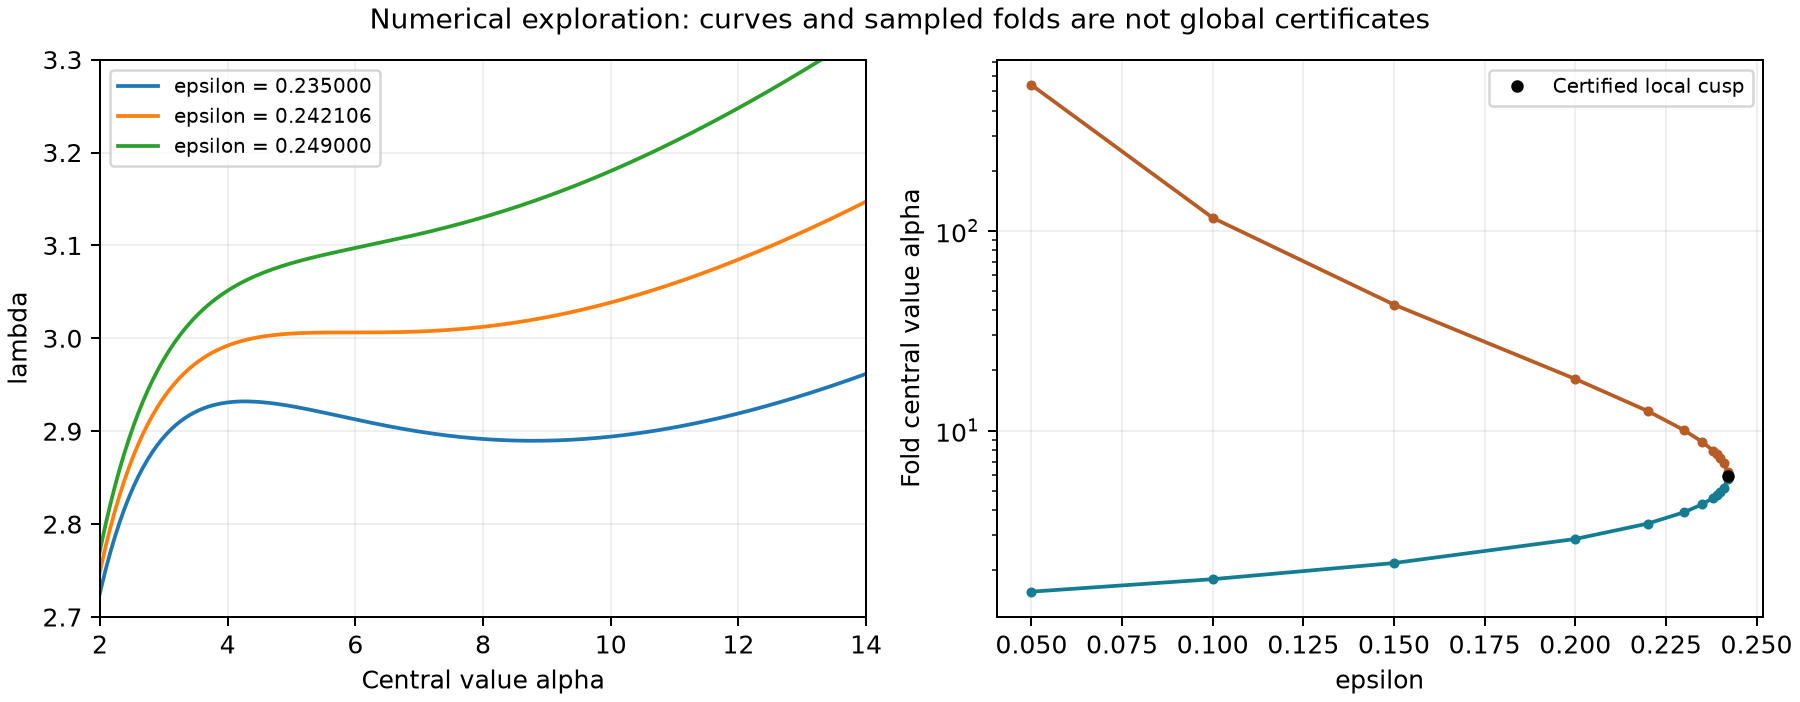
\includegraphics[width=\linewidth]{figures/exploration.png}
\caption{Non-rigorous shooting curves and sampled folds. These illustrations
are separate from the local cusp and global interval certificates.}
\end{figure}

From this problem folder, in an environment with python-flint and SymPy, run
\begin{verbatim}
python scripts/check_analytic.py
python scripts/validated_cusp.py
python scripts/validated_reduced.py --full --workers 6
\end{verbatim}
Every certification check prints PASS or FAIL; a failure exits nonzero.
Both validators recompute all enclosures rather than trusting saved JSON
files. The local input is \texttt{certificates/cusp-input.json}; its output is
\texttt{certificates/cusp-certificate.json}. That computation takes about
40 seconds on one thread. The global cover takes about 145 seconds with six
single-thread numerical processes and produces
\texttt{reduced-cover.json} in the certificates folder. Exact timings are recorded in the
JSON outputs. SciPy is used by the global script solely to propose rational
event windows; it is not part of the trusted enclosure arithmetic.
The successful logs are \texttt{certificates/validation.log} and
\texttt{certificates/reduced-validation.log}. Arithmetic decisions use Arb;
the implementation, Arb/FLINT and their arithmetic dependencies are part of
the trusted computing base. No interval input is inferred from a plotted curve.
The optional exploration and plotting scripts take about 30 and 10 seconds.
The API audit requires network access and is not a mathematical certificate.
The manuscript is compiled with the repository's shared preamble and build script.

\section{Verification status and dependencies}
The argument covers all $\varepsilon>0$ and all positive amplitudes; no
parameter gap remains in the stated proof.

An independent verifier (Claude Opus 5.5, fresh context, no access to the
solver's reasoning) checked the hypotheses of KLO Theorems 3.1 and 4.1 and of
the corresponding original statements of Du and Lou, re-derived the reduction,
the equivalence \eqref{eq:foldlevel}, the signs in \eqref{eq:Ederiv}, the
Wronskian arguments and the tail exclusion, and re-ran the three certificate
scripts, which reproduce the delivered certificates. With a separate
implementation (Julia, IntervalArithmetic.jl, parameter derivatives carried as
3-jets, a real-variable bootstrap at the origin, automatic event windows) the
verifier re-certified the pattern of signs on $[1/2,8/5]$ with 564 boxes, the
three point values \eqref{eq:levels}, and, in the reduced variables alone,
the enclosures of $\varepsilon_0$, $\alpha_c$ and $\lambda_c$ of
\zcref{thm:local}; its 160-bit enclosure
$\varepsilon_0\in[0.24210616559523735,\,0.24210616559523776]$ is sharper than,
and contained in, the one stated above. Details and the remaining reservations are in
\texttt{verification.md}; the verifier's scripts are in \texttt{verification/}.
The status is \emph{solved}. The novelty audit is a bounded literature search.
Arb/FLINT, IntervalArithmetic.jl and the two implementations belong to the
trusted computing base.

\clearpage
\paperreferences
\end{document}
